\section{On the Human Soul}

\textit{St Gregory of Nyssa on the Human Soul} by \textsc{John P. Cavarnos}, Edited and Revised by \textsc{Constatine Cavarnos}, 95 pp, Institute for Byzantine and Modern Greek Studies\footnote{\url{http://ibmgs.org/}}

\begin{quotex}
We regard all knowledge as beautiful and precious, but one kind of it more so than another, either by reason of its exactness, or because it has reference to superior and more wonderful objects. On both these accounts we should naturally be led to place in the front rank the study of the soul. \flright{ \textsc{Aristotle}, \emph{On the Soul}} 

\end{quotex}

Originally published as a doctoral dissertation, this edition was revised for use by a more general audience. Since the fundamental goal of Christianity is the “salvation of souls”, it is curious that there was no systematic understanding of the soul until the efforts of \textbf{St Gregory of Nyssa}. Mr. Cavarnos points out:

\begin{quotex}
Christianity, being concerned above all with man's destiny and salvation, must inevitably undertake to explain the mystery of life. For the Christian that means more specifically the human soul. 

\end{quotex}
Curiously, St Gregory turns to the great pagans of antiquity, in particular \textbf{Plato} and \textbf{Aristotle}, for his understanding of the soul. There are a few explanations that have been proposed by Gornahoor. The first is attributed to \textbf{Julius Evola}, who would regard this as the process of “rectification”, i.e., the partial restoration of the Middle Ages to its pagan roots following the shock of primitive Christianity. \textbf{Guido De Giorgio}, on the other hand, would regard the two Romes — the Ancient and the Medieval — as two forms of the same tradition, the later a deepening of the earlier. Our preference is that St Gregory is giving us a guidebook to the soul, not a theory, and anyone who makes the efforts at self-knowledge will simply see that it is true.

\begin{wrapfigure}{tr}{.3\textwidth}
 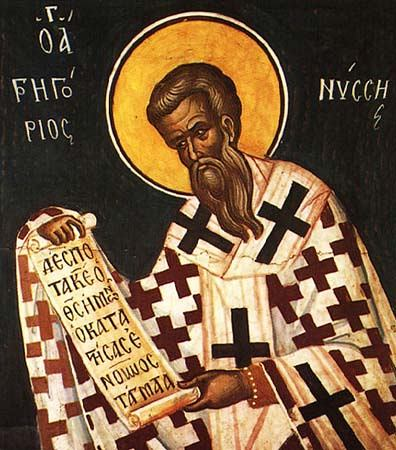
\includegraphics[scale=1]{a20130315OntheHumanSoul-img001.jpg} 
\end{wrapfigure}

Unfortunately, Mr. Cavarnos falls prey to the modernist notion that St Gregory was merely making “good use of classical and contemporary material for giving form and expression to accepted Christian doctrines and concepts.” Were that true, then why couldn't modern theories of the mind or soul be put to the same use? No, it is not a pragmatic concern for good usage, but whether the doctrine is true or not.

\paragraph{Anthropology}
Like the pagan philosophers, St Gregory conceived the cosmos as divided into two orders: the spiritual and rational over against the material and irrational. In his understanding of the purpose of man, St Gregory is closer to his Christian roots. Mr. Cavarnos summarizes:

\begin{quotex}
Man was created in the image and likeness of God so that he could partake of the divine nature and make it known to the rest of the creation. He is related to God by his endowment of the divine principle of reason, through which he knows God and imitates Him to attain to virtue and perfection. 

\end{quotex}
So man is suspended between the two poles and is to be the link between them. Following \textbf{Rene Guenon}, we have referred to those poles as form and matter, or essence and existence. The former binds man with the divine and the latter with the subrational world. In his higher role, man possesses divine attributes such as life, reason, wisdom, and so on. Man is also a microcosm, so his self-knowledge relates to the knowledge of the cosmos by analogy.

\paragraph{Nature of the Soul}
St Gregory makes a useful distinction of his study. The metaphysics of the soul relate to the essence, origin, and destiny of the soul, and the psychology of the soul is concerned with determining, defining, and classifying the diverse faculties of the soul. This psychology is necessarily a phenomenology, since the soul can only be directed observed from the inside.

Starting with the nature of the soul he claims that the soul is the principle that gives life to the body. That is, it animates the body, from the Latin word anima for soul. Immediately, this is the opposite of educated men today who believe, on the contrary, that the soul is a function, or epiphenomenon, of the body. Not so, and this is why Rene Guenon identifies the five fundamental preconditions for manifestation: space, time, form, matter, and life. Hence, there are both material forces and psychic forces in play, irreducible to each other. Evola makes use of this idea in his own doctrine of the degrees of race. Of course, these are the natural forces, which operate on the horizontal plane, and not the supernatural, or vertical, forces.

St Gregory, like Plato, accepts the immortality of the soul as well as its simplicity. Mr. Cavarnos does not point this out, but this is analogous to the Roman idea of divine simplicity, which should be expected if the soul is truly the likeness of the divine. In this case, the human soul is chiefly identified with the rational, or intellectual, faculty; this faculty is therefore the ruling principle. Again, this is consistent with the ancient pagans and the Medieval tradition.

Gregory brings up an excellent and very important point: the “passions” are actually distinct from the soul, hence cannot be considered part of it. For Gregory, the soul is beautiful, which would preclude any ugliness. This means two things in practice:

\begin{itemize}
\item Man's interiority is subject to inferior and subrational influences arising, as it were, from outside of himself 
\item When a man submits to the demands of these influences, he is not fulfilling himself, but, on the contrary, he is surrendering up his self to an outside agent 
\end{itemize}
Gregory, like St Anthony of the Desert\footnote{See Section~\ref{sec:St Anthony and Practical Reason} of this book.}, regards these passions as animal traits. These are the beasts of the field that must be named and mastered. The questions that we brought up at one point are worth revisiting: if a being is dominated by his passions, to what extent can he be considered as a man rather than an animal? On one hand, the case can be made that he is a “virtual” man, since he has the possibility of being rational.

\paragraph{The Origin of the Soul}
Gregory rejects two doctrines: the preexistence of the soul and the theory of reincarnation. Like contemporary writers on tradition, Gregory demonstrates the metaphysical impossibility of reincarnation, with an argument that doesn't need to be discussed at the moment. Keeping in mind Aristotle's five versions of priority, Gregory rejects the temporal preexistence of the soul, but not the ontological preexistence.

For Gregory, the whole of humanity preexisted in God's mind as a possibility, not an actuality. Clearly, this is consistent with what Guenon writes in the \emph{Multiple States of Being}. A soul is a possibility of manifestation. Gregory accepted traducianism (the rational soul is passed in the semen), which is hard to defend, as it makes of it a natural process. In keeping with traditional metaphysics, the soul manifests in a world in which it is compossible with the rest of the world. That is, the soul manifests when there is an affinity between the possibilities of the soul and the particular world in which those possibilities can be actualized. I'm sorry that his cannot be proved in the manner of the geometers, but a man can just “see” that it is so, provided he has sufficient self-knowledge.

Like \textbf{St Thomas Aquinas} after him, Gregory claims that the soul passes through three stages: the insensible stage, the sensible stage, and the rational stage. Since the soul is the form of the body,

\begin{quotex}
the soul is the determining principle or cause in the living being. It constructs for itself a body that is suitable, like a seal that impresses its stamp on wax. 

\end{quotex}
Once again, this is an idea that has been insufficiently developed. It seems, therefore, that the features of a man's body are not accidental, incidental, arbitrary, irrelevant, or unimportant. Rather they are the visible manifestations of the invisible soul. We will explore this idea further in the mailing list.

\paragraph{The Soul after Death}
Plato, Origen, and the Bible provided the sources for Gregory's thought on this matter. Unlike the fundamentalists of today — and I would include the anti-Christian, neo-Nietzschean and neo-pagans in that camp — Gregory tends to understand Scripture allegorically rather than literally. Gregory believed that by the very order of things, the good and justice will ultimately prevail. Again, this is consistent with Guenon in the \emph{Symbolism of the Cross}. Gregory believed that if the soul becomes mindful of its previous sins, and fearful of their consequences, he becomes wise and prudent. That is a big “if”. On the one hand, few today believe they are sinful or that there are consequences. On the other hand, the neo-Christians who believe in “faith alone”, don't accept that there is any necessary reason to become wise or prudent.

I will gloss over the discussion of the resurrection, but will point out that “resurrection is the restoration of our nature to its original state.” Of course, for us, that is the Primordial State. In that state, there is no childhood, old age, disease, or infirmity. The body is incorruptible and is finer and lighter. This is not unlike what Guenon wrote about the body being lighter in earlier yugas. Obviously, the impure souls will not be part of this resurrection to the Primordial State.

\paragraph{The Relation of Body and Soul}
Gregory claimed that

\begin{quotex}
the study of the soul and its relation to the body is of primary importance, since the knowledge of the soul and the manner in which it operates in the body has a profound bearing on the ideas of perfection and salvation, as well as on man's well-being and thinking. 

\end{quotex}
If that be so, then why does no one in the West consider it very important? Only in the East, do some men continue to map out the intricacies of the soul. If Gregory is correct, then we understand why Protestantism is so destructive, since salvation, for it, involves little more than responding to an altar call.

Unlike the pagans, like Plotinus for example, who regarded matter as inherently evil, Gregory saw the origin of sin in man's will, not in the body, per se. Nevertheless, the lower forces, which as we pointed out earlier arise from the outside of man, must be overcome. Specifically, men in the flesh must separate or detach from such forces. This does have an effect on salvation:

\begin{quotex}
if anyone is entirely preoccupied with the things of the flesh and uses every movement of the soul and all its energy for his fleshy desires, he will not be separated form experiences involving the flesh, even when he is out of it. 

\end{quotex}
Gregory has an interesting understanding of the senses:

\begin{quotex}
Since the senses are more akin to the coarseness and earthiness of the body than to the soul, they are subject to errors. They are termed windows through which death enters, for they lead men to the life of the passions and bodily pleasures. 

\end{quotex}
Men today are in basic agreement, except that for them life enters through the senses. Sensuality is considered normal and good. For the moderns, the purpose of the intellect is to think up ways to improve sensual experience: the body desires and the soul tries to satisfy it. For Gregory, the reality is reversed: the body is the instrument of the soul. The soul commands and the body executes. This is not life denying, since the intent is not to cause the body to suffer, but rather to improve the life of the soul. The desires of the body are never fully sated, so men today are anxious, angry, fearful and seek to hide from them through the pursuit of “good” experiences. Rather, the soul should learn to be ordered, just as the macrocosm is ordered.

\paragraph{The Faculties of the Soul}
\subparagraph{The Platonic Element}
Gregory follows Plato's naming of the three powers of faculties of the soul:

\begin{itemize}
\item Nous. The rational power consisting of intellect and will. 
\item Thymos. The spirited or striving faculty. 
\item Epithymia. The appetitive faculty of desire. 
\end{itemize}
Gregory says the inclinations of thymos and epithymia are harmful or good, depending on how they are applied. Although they are beast like, they cannot be reduced to instincts, presumably because instincts are mechanical and, as such, are beyond ordinary conscious control.

When under the dominion of the nous, of the two lower faculties, one gives courage and the other the desire to participate in the good. Otherwise, disorder sets in. Gregory's teaching is summarized in Table~\ref{tab:On the Human Soul}.

\begin{table}[h]\small
\begin{tabular}{lll}\toprule
\textbf{Faculty} &
\textbf{Virtue} &
\textbf{Illness}\\\midrule
Rational & Contemplation of the divine & Impiety\\
& Discernment between good and evil& Lack of sound judgment \\
&&concerning the truly good\\
&Clear and unconfused knowledge  & False opinion regarding \\
&of physical nature&the nature of things\\\midrule
Spirited & Hatred of evil &Envy\\ 
& The struggle against passions & Hatred \\
& The urging of the soul to courage & Malice \\\midrule
Appetitive & The virtuous motion toward & The love of money \\
&what is worth desiring&\\
& An erotic impulse towards virtue & Sensuality
\\\bottomrule
\end{tabular}
\caption{Powers of the soul according to Plato}
\label{tab:On the Human Soul}
\end{table}

\subparagraph{Disorders of the Rational Faculty}
Although most people focus on the illnesses of the spirited and appetitive faculties, it is actually the illness of the intellect which is more serious and the most difficult to eradicate. A man who is disordered in his spiritedness or appetite can learn to overcome them, provided his intellect is still sound. Unfortunately, a man with a disordered intellect is not even aware of this disorder; hence, he has no incentive to change. These types of men make communication difficult.

It is worth the effort to update Gregory's symptoms. Now, as then, impiety is a common illness of the rational soul. Impiety means the denial of the existence of any higher, spiritual influences; moreover, any such teachings are simply mocked.

Lack of judgment of the good leads to regarding the disorders of the lower faculties as good, rather than the bad that they really are. Or things that are necessary are regarded as evil. This leads to a strange kind of neo-Puritanism. Although I'm not an advocate of Puritanism, at least their intent was to establish order and lead to salvation after death. Neo-Puritanism, on the contrary, seeks to abolish death, an obvious absurdity. This leads to public attacks on smoking, the right to bear arms, and even on what the populace is allowed to eat and drink.

The disease of misunderstanding the nature of things leads to decision-making base on sentimental motives or wishful thinking, rather on how things really are. Anyone who opposes such beliefs is shamed, ostracized, or even worse, if they hold positions of power.

As we have pointed out, the roots of these errors go deep and are based on the rejection of one or more metaphysical principles. For example, we have shown how the rejection of final or formal causes leads to specific sorts of errors. The rejection of order, i.e., impiety, leads to Marxist-like plans to overturn the established order.

\subparagraph{The Aristotelian Element}
Alongside the Platonic understanding of the soul, Gregory also draws on Aristotle. For him, they are not in contradiction. Gornahoor would say that the Platonic understanding is founded on interiority and is proved by the dominion of the rational soul.

The Aristotelian perspective starts from the senses and leads inward. So he accepts the understanding of the soul as encompassing three elements:

\begin{enumerate}
\item The vegetative soul, which controls growth and increase and the activities of life. 
\item The sensitive soul, which governs sense activities. 
\item The rational soul, or intellectual power 
\end{enumerate}
Gregory writes:

\begin{quotex}
The perfect life in the body is seen to be in the rational nature of man, being nourished and perceived by the mind, participating in reason and governed by the mind. 

\end{quotex}
In keeping with the outer orientation, the nous, or rational soul, exteriorizes its activities in matter. Thus, the nous is united to power, which is the ability to bring ideas and plans into manifestation. Since the soul is beautiful, what it makes manifest will also be beautiful.

\paragraph{Free Will and Virtue}
In the final chapter, Mr. Cavarnos addresses Gregory's teaching on the will. He defines freedom:

\begin{quotex}
freedom is choosing freely the object desired. Will is a faculty exempt from servitude, free, residing in the independence of our reason. Free will is the essential foundation for virtue, for if it is lacking, then there can be no virtue, no praise, no blame for human conduct. 

\end{quotex}
The consequences of this teaching are hard, and few are willing to accept it. Gregory explains:

\begin{quotex}
The soulless or irrational beings are led by an external will. If a rational and thinking nature discards freedom, it also loses the right for thinking. 

\end{quotex}
Obviously, a multitude of spiritual influences abound, whose goal is to implant themselves in unaware minds, thus controlling their wills in a very real sense. Isn't this far too obvious to deny? For example, in the USA, almost out of nowhere, a movement arose to infringe the right to bear arms. Suddenly the nation was mobilized, the media focused on the topic, the populace talked about it, and so on. The “debates” on the topic are almost always reduced to swapping slogans or making sentimental arguments. I saw one woman saying, in all seriousness, that women don't need a gun for self-defense since she “feels” safe even when walking in bad neighborhoods. Apparently, any argument — whether pro or con — is unnecessary, since her feelings trump any such argument.

I am not trying to adjudicate that issue here, but to point out how external ideas take hold in a mind. This irrationality is considered “soulless” by Gregory. As you go through the day, can you tell which beings that you encounter actually have a soul and which are soulless?

According to Gregory, God endowed human nature with the principle of all that is beautiful, and the most precious and beautiful good is the gift for being independent and free. Necessity and compulsion negate man's being the image of God.

Hence, when a man makes a bad choice, he must accept the consequences of that choice. This is the natural result and not a special act of divine retribution as some are inclined to think. The conclusion from this is clear, as was shown in Guido De Giorgio's meditation on death\footnote{\url{https://www.gornahoor.net/?p=11683}}. God does not directly punish a soul, or send it to hell or whatever other place or state; rather, man himself chooses his own ultimate state.

Mr. Cavarnos does not draw any conclusions from this; nevertheless, Gornahoor thinks there is a clear and important conclusion. If all this is true, then the salvation of the soul requires the development of the rational faculty or nous. This is measured in several ways:

\begin{itemize}
\item The rational soul becomes the master of the lower faculties. 
\item It contemplates the divine 
\item It discerns between good and evil 
\item It has clear knowledge about physical nature 
\item It exteriorizes itself in a life of virtue and beauty 
\end{itemize}

\flrightit{Posted on 2013-03-14 by Cologero}